\section{Tuning General Parameters}
\label{sec:prep}

The main research topic of this thesis is to find out which variation of genetic algorithms works best in solving the TSP. In order to provide an answer, this chapter considers first how the initial population can be constructed and which settings for the general parameters should be used. \par 

\subsection{Preliminaries}
\label{subsec:prep}

We used the symmetric instances of the TSPLIB library (see \cite{TSPLIB}) for our experiments. Since this dataset uses a variety of different file formats, it was necessary to make some preprocessing steps and create a unified format to work with the data. We assume that the number of cities can influence the performance of our genetic algorithm; therefore, we have divided the data into five groups of similar size:

\begin{itemize}
	\item TSP instances with less than 100 cities (22), 
	\item TSP instances with 100 to 200 cities (24),
	\item TSP instances with 200 to 500 cities (18),
	\item TSP instances with 500 to 1500 cities (23), and
	\item TSP instances with 200 to 500 cities (15).
\end{itemize}	

Some of the instances have a known optimal solution which can serve as a benchmark in the experiments. Let $f_{i}$ be the fitness value of the chromosome returned by the genetic algorithm for a TSP instance $i$ and $f_{i}^{opt}$ be the fitness value of the chromosome which encodes an optimal tour for $i$. In order to measure the effectiveness of different operators in our genetic algorithm, we introduce the index:

$$E_{opt}(i) = (f_{i}^{opt} - f_{i})/f_{i}^{opt}$$ 

This index corresponds to the relative error of the fitness value $f_{i}$ with respect to the optimal value $f_{i}^{opt}$. Moreover, we denote by $E_{opt}^{t}$ the average of $E_{opt}(i)$ over $t$ instances. A most effective configuration of the genetic algorithm is one which minimizes $E_{opt}^{t}$.\par 

 Most of the TSP instances come however without an optimal solution. Moreover, the used library (see \cite{TSPLIB}) does not provide any information about the best known solutions for these instances as well. Therefore, for these instances, the results of our experiments will be compared to the solutions provided by construction heuristics. Therefore, we introduce the index: 
 
 $$E_{h}(i) = (f_{i}^{h} - f_{i}) /f_{i}^{h}$$ 
 
 $f_{i}^{h}$ is the fitness value of the chromosome which encodes a shortest tour delivered by construction heuristics within ten minutes. This index corresponds to the relative error of the fitness value $f_{i}$ with respect to the fitness value $f_{i}^{h}$. Moreover, let $E_{h}^{t}$ be the average of $E_{h}(i)$ over $t$ instances. A most effective configuration of the genetic algorithm is one which minimizes $E_{h}^{t}$. For the cases where the genetic algorithm shows better results than the heuristics, we will use another index: 
 
 $$I_{h}(i)  = (f_{i} - f_{i}^{h})/f_{i}^{h}$$
 
This index corresponds to the improvement made by the genetic algorithm over $f_{i}^{h}$. $I_{h}^{t}$ is an averaged $I_{h}(i)$ over $t$ instances. We want to maximize $I_{h}^{t}$.\par 

Please note that all the following experiments have been conducted using a Genuine Intel CPU $@1601.320 MHz$ with 9 GB memory. In each experiment, the genetic algorithm has a time limit of ten minutes. The program code and all the raw data are available in \cite{Bechberger2020}.\par 

As already mentioned in Section \ref{subsec:ga}, there are two main ways to construct an initial population, namely, randomly or using heuristics. We are going to use both variants in our experiments. We have implemented the following construction heuristics: nearest neighbor (see Section \ref{subsec:nn}), double nearest neighbor  (see Section \ref{subsec:dnn}), nearest insertion (see Section \ref{subsec:ni}), and farthest insertion (see Section \ref{subsec:fi}). All of these heuristics are deterministic, but their results may depend on the start city. In order to initialize the population, we repeatedly ran each heuristic with a new randomly drawn start city until a given time limit of ten minutes was reached. This was done for each TSP instance individually. In the best case, the number of different tours is equal to the size of the TSP instance. Naturally, some of the tours which will be produced by the heuristics represent the same tour. We only include the chromosomes containing different tours in the initial population.\par

Please note that the above mentioned heuristics were launched separately from the genetic algorithm. During ten minutes, we sequentially started one heuristic after another with a randomly drawn start city. When ten minutes ran out, we stored the results to use them in our genetic algorithm. Thus, the time needed for the random initialization of the population does not significantly differs from the time needed to initialize the population using the results of heuristics. If the number of different tours provided by the heuristics is smaller than the desired population size, the remainder of the population is filled with random permutations of the cities. We also ensure that these random chromosomes represent different tours.\par 

In addition to this heuristic-based initial population, we will also consider an initial population which does not contain results of the heuristics, that is, which is exclusively based on random permutations.

\subsection{Experimental Setup}


In our first experimental step, we want to analyze which configuration of two general parameters, namely population size and mutation rate, results in the best performance.  In order to do so, we will study how the fitness value changes when varying these parameters while keeping the type of crossover, selection and mutation fixed. We have chosen the order crossover because, according to the literature (e.g., see \cite{starkweather1991comparison}), it has shown better results than the other path representation crossover operators. Moreover, the edge preserving operators (AEX, ERX, and HX) cannot find good solutions for larger TSP instances according to \citeauthor{potvin1996genetic} \cite{potvin1996genetic}. Among the mutation operators, we have chosen the shift mutation as it works on the whole chromosome and not only on a part of it. We therefore assume that it may result in larger changes. Finally, the tournament was chosen as selection operator, as it is easy to implement and gives good results (see Section \ref{subsec:tournament}). \par 

We have considered two groups of TSP instances:

\begin{itemize}
	\item TSP instances with less than 100 cities, and
	\item TSP instances with 200 to 500 cities.
\end{itemize}	

The motivation for this choice is that the instances are still small enough so that we can provide quite a large number of iterations. Besides, we assume that best configurations of parameters in these two groups could differ. Therefore, the experiments will be made for each group of instances separately.\par

As it was highlighted by \citeauthor{zhang2010effects} \cite{zhang2010effects} who analyzed the effects of population size on the performance of genetic algorithms, "we do not have any reliable theory for choosing $N$", where $N$ is the population size. The choice of an adequate population size can be difficult. On the one hand, if the size of the population is set too small to decrease the costs of calculations, the genetic algorithm has a poor choice of chromosomes which it can use; therefore, it can be hard for the genetic algorithm to find chromosomes with a good fitness value. On the other hand, very large populations can cause very high processing time and very slow convergence. \par 

The common practice for setting the size of the population consists of using fix numbers like 20, 100, 200, 300, and 500 (\citeauthor{zhang2010effects}, \cite{zhang2010effects}) or 1000, 5000, and 10000 (\citeauthor{rexhepi2013analysis}, \cite{rexhepi2013analysis}) without considering the size of the TSP instances used in experiments. As one can see, the numbers used by different researchers are quite different; therefore we would like to use another approach inspired by \citeauthor{chen2015measuring} \cite{chen2015measuring}. They investigated the curse of dimensionality in population-based algorithms and suggested to take into consideration the size of an instance when defining the population size. They do so by introducing a population size factor. Multiplying this factor with the size of an instance results in the size of the population. Although their research was conducted on particle swarm optimization and differential evolution algorithms, this approach can be used for genetic algorithms as well. \par 

For both groups of instances we consider, it is possible to set the size of the population larger than the tour length to provide diversity in the population. Setting it smaller or even equal to the number of cities did not show promising results for both groups in preliminary investigations. A single iteration for this group of instances takes very short time. As a result, the genetic algorithm can produce a great number of iterations and slow convergence is therefore not expected to be a problem here. Thus, we consider the following options for the size factors $s$ which is multiplied with the number of cities to obtain the population size: $s_{1} = 3$,  $s_{2} = 5$. 

Let us now consider the second general parameter, namely the mutation rate. There are several studies trying to optimize this hyperparameter, including the study by \citeauthor{beed2017study} \cite{beed2017study} about defining the GA parameters for solving Multi-Objective TSP. They considered mutation rates of $1\%$, $3\%$, $5\%$, and $10\%$. A mutation rate of $1\%$ did not show promising results on our instances in preliminary experiments and was excluded from our further consideration. We therefore use the following mutation rate values $m$ in our analysis: $m_{1} = 3\%$, $m_{2} = 5\%$, and $m_{3} = 10\%$.

Overall, we thus have $2 * 3 = 6$ possible combinations for mutation rate and size factor. However, before analyzing them, we have conducted one more small preliminary experiment with respect to the tournament selection. We used the instances of the first group (with less than 100 cities), took these 6 combinations of mutation rate and size factor and considered three variants for the number of participants $p$ in the tournament: randomly chosen from a small interval [2, 10], fixed at the expected value of this interval, namely 6, and fixed at a smaller value 3.\par  

After that, we conducted a grid search on parameter settings for size factor and mutation rate evaluating all 6 possible combinations. So we used the following setting for our genetic algorithm:
\begin{itemize}
	\item order crossover,
	\item shift mutation with the mutation rate $m$, where $m \in \{3\%, 5\%, 10\%\}$,
	\item tournament selection with the number of participants to be defined in a preliminary experiment,
	\item population size factor $s$, where $s \in \{3, 5\}$, and
	\item a time limit of ten minutes.
\end{itemize}

The experiments in this step were conducted without using heuristics in the population, that is, the population was initialized with random permutations. This choice was motivated by the results of several preliminary trials, where the heuristics were used: For some small instances with less than 100 cities the heuristics achieved the optimal values  and for many instances of this group were close to the optimum; therefore, the results of different configurations for genetic algorithm showed similar results and could not be compared properly.  \par 

 Please note that as genetic algorithms are nondeterministic, each configuration is always launched with 3 different seeds. The results are averaged over these three runs.\par 


\subsection{Results and Discussion}
\label{subsec:parameters_results}

 \begin{figure}[htp] \centering
	\begin{subfigure}[t]{0.45\textwidth}
		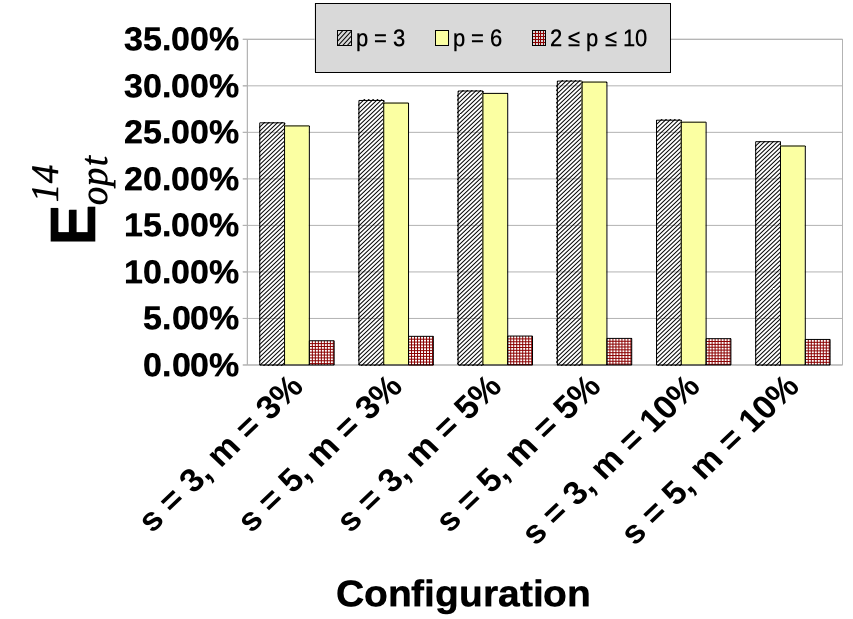
\includegraphics[width=\textwidth]{8_3_selection_number_vs_opt}
		\caption{Relative error with respect to the optimal value averaged over 14 instances.}
		\label{fig:8_3_selection_number_vs_opt}
	\end{subfigure}
	\hfill
	\begin{subfigure}[t]{0.45\textwidth}
		\centering
		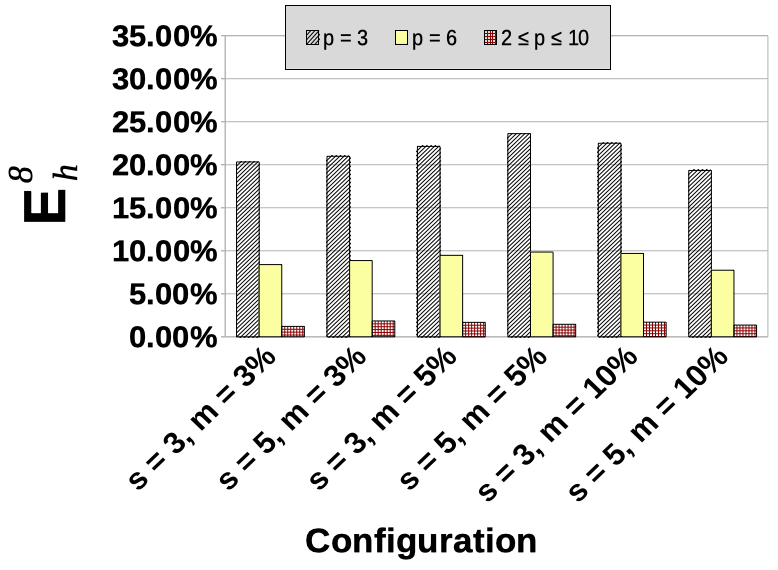
\includegraphics[width=\textwidth]{8_3_selection_number_vs_h}
		\caption{Relative error with respect to the best results of heuristics (with ten minutes limit) averaged over 8 instances.}
		\label{fig:8_3_selection_number_vs_h}
	\end{subfigure}	
	\caption{Relative error for 22 instances with less than 100 cities for 6 settings of general parameters and different variants of the tournament selection.}
	\label{fig:8_3_selection_number}
\end{figure}
	
Concerning the number of participants for the tournament selection, the first option where we used a random number drawn from the interval [2, 10] showed the best results (see Figure \ref{fig:8_3_selection_number}); therefore, we will use this approach.\par

\begin{figure}[htp] \centering
	\begin{subfigure}[t]{0.45\textwidth}
		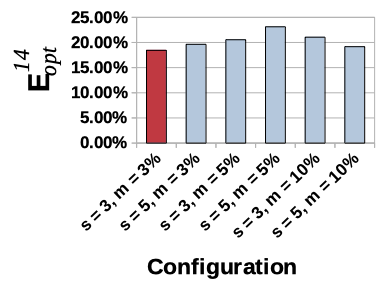
\includegraphics[width=\textwidth]{8_3_vs_opt_less_100}
		\caption{Relative error with respect to the optimal value averaged over 14 instances.}
		\label{fig:8_3_less_100:vs_opt}
	\end{subfigure}
	\hfill
	\begin{subfigure}[t]{0.45\textwidth}
		\centering
		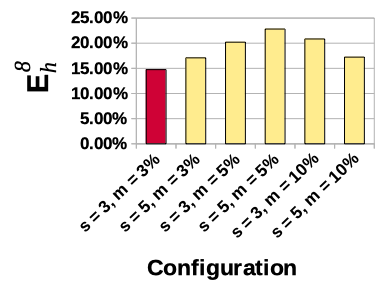
\includegraphics[width=\textwidth]{8_3_vs_heuristics_less_100}
		\caption{Relative error with respect to the best results of heuristics (with ten minutes limit) averaged over 8 instances.}
		\label{fig:8_3_less_100:vs_heuristics}
	\end{subfigure}	
	\caption{Relative error for 22 instances with less than 100 cities for 6 settings of general parameters.}
	\label{fig:8_3_less_100}
\end{figure}

Now, we look for the best combination of parameters for two groups of instances, namely for the ones with less than 100 cities and the ones with 200 to 500 cities. For the group of instances with less than 100 cities, the combination $s = 3, m = 3\%$ showed the best results for both indices $E_{opt}^{14}$ and $E_{h}^{8}$ (see Figure \ref{fig:8_3_less_100:vs_opt} and Figure \ref{fig:8_3_less_100:vs_heuristics}). 

\begin{figure}[htp] \centering
	\begin{subfigure}[t]{0.45\textwidth}
		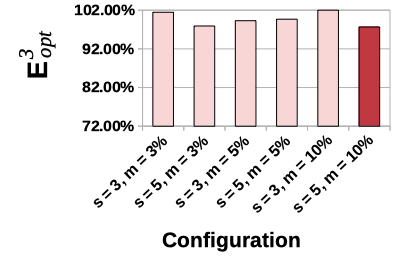
\includegraphics[width=\textwidth]{8_3_vs_opt_200_to_500}
		\caption{Relative error with respect to the optimal value averaged over 3 instances.}
		\label{fig:8_3_200_to_500:vs_opt}
	\end{subfigure}
	\hfill
	\begin{subfigure}[t]{0.45\textwidth}
		\centering
		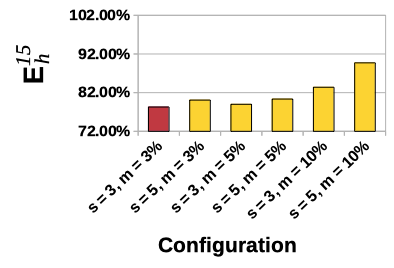
\includegraphics[width=\textwidth]{8_3_vs_heuristics_200_to_500}
		\caption{Relative error with respect to the best results of heuristics (with ten minutes limit) averaged over 15 instances.}
		\label{fig:8_3_200_to_500:vs_heuristics}
	\end{subfigure}	
	\caption{Relative error for 18 instances with 200 to 500 cities for 6 settings of general parameters.}
	\label{fig:8_3_200_to_500}
\end{figure}

For the group of instances with 200 to 500 cities there are only 3 instances with a known optimal value. For them, the best configuration was $s = 5, m = 10\%$ (see Figure \ref{fig:8_3_200_to_500:vs_opt}). 
The other 15 instances have no known optimal value. Their results with respect to the best results of heuristics showed that the configuration $s = 3, m = 3\%$ was the best (see Figure \ref{fig:8_3_200_to_500:vs_heuristics}). \par

The differences among the configurations for the first group with less than 100 cities were much smaller as for larger instances of the second group with 200 to 500 cities. So, perhaps, the choice of such parameters as mutation rate and population size plays a more important role for larger instances.\par  

The best configuration was different only for the case with 3 instances within the group with 200 to 500 cities, while for all other instances the same configuration, namely $s = 3, m = 3\%$, was the best. We consider the different result of these three instances as an outlier and choose the configuration $s = 3, m = 3\%$ to work with further because it worked at best for the most instances. \par  

It is interesting to mention that while for smaller instances with less than 100 cities the error was smaller than $25\%$, for larger instances with 200 to 500 cities, the error exceeds $75\%$. This can be explained by the fact that the genetic algorithm completes less iterations in case of larger instances; therefore, it has not enough time to come to better solutions as it can do for smaller instances.\par 

\begin{table}[htp] \centering
	\centering
	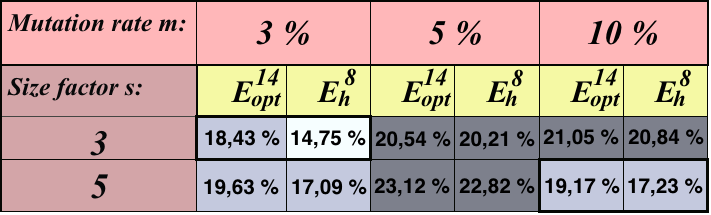
\includegraphics[width=0.5\textwidth]{tab_8_3_parameters}
	\caption{Results for six combinations of general parameters for instances with less than 100 cities.}
	\label{Tab:tab_8_3_parameters}
\end{table}

As there are significant differences in $E_{opt}$ and $E_{h}$ between two groups of instances, it makes sense to continue comparing the results among different size groups and not averaging over all instances.\par 

Finally, if we take a look at Table \ref{Tab:tab_8_3_parameters}, we can see that for small mutation rates like $3\%$, a smaller size factor is better. At the same time, for large mutation rates like $10\%$, a larger size factor performs better. This means that if there occur many mutations, the population has to be large, at least for small instances with less than 100 cities.\par 